\chapter{Neuronale Netze in Tensorflow}
Neuronale Netze sind das am h\"aufigsten benutzte Werkzeug in Tensorflow. Im Folgenden werden die Grundlagen f\"ur Neuronale Netze vorgestellt, sowie deren Umsetzung in Tensorflow. Diverse Codeauschnitte in diesem und allen nachfolgenden Kapiteln sind Implementierungen in der Programmiersprache Python. Diese werden in den Pythoncode eingebunden. Dabei wird mit \cite{cookbook}
\begin{lstlisting}
import tensorflow as tf
\end{lstlisting} Tensorflow in Python importiert. Tensorflow-Befehle können dann über das Kürzel \lstinline$tf.$ aufgerufen werden.

\section{Feedforward Netzwerk}
Die h\"aufigste in Tensorflow implementierte Version Neuronaler Netze ist das feedforward network oder ein vorwärtsgerichtetes Netzwerk. Der Name stammt von den Informationen, die innerhalb des Netzes immer weiter nach $"$vorne$"$ wandern, von den Eingabeneuronen über die versteckten Schichten zu den Ausgabeneuronen.\cite{Goodfellow} Es gibt keine Rückkopplungen, wie es zum Beispiel beim Hopfieldnetz der Fall ist.\cite{Ertel2013} Sie werden in der Regel f\"ur Deep Learning verwendet.\cite{Goodfellow} Ein feedforward Netz besteht aus einer Eingabeschicht, einer Ausgabeschicht und n versteckten Schichten dazwischen.
\begin{figure}[!htp]
	\setlength{\unitlength}{1cm}
	\centering
	\begin{picture}(4,3.5)
	\label{FeedForward}
	
	\put(-0.2,0.5){\textcolor{blue}{$w_{1,1}$}}
	\put(1.35,0.26){\textcolor{blue}{$w_{2,1}$}}
	\put(2.8,0.2){\textcolor{blue}{$w_{n,1}$}}
	\put(4.1,0.6){\textcolor{green}{$w_{n,{m_1}}$}}
	
	\put(0.53,-0.1){$x_1$}
	\put(2.05,-0.1){$x_2$}
	\put(3.54,-0.1){$x_n$}
	\put(4.5,-0.1){\textbf{Inputschicht}}
	
	\put(0.75,0){\circle{0.5}}
	\put(2.25,0){\circle{0.5}}
	\put(3.75,0){\circle{0.5}}
	
	\put(0,1.5){\circle{0.5}}
	\put(1.5,1.5){\circle{0.5}}
	\put(3,1.5){\circle{0.5}}
	\put(4.5,1.5){\circle{0.5}}
	\put(5.25,1.35){\textbf{Versteckte Schicht}}
	
	\put(1.5,3){\circle{0.5}}
	\put(1.3,2.9){$o_1$}
	\put(3,3){\circle{0.5}}
	\put(2.8,2.9){$o_2$}
	\put(4.05,2.85){\textbf{Outputschicht}}
	
	\put(0.75,0.25){\textcolor{blue}{\line(-3,5){0.63}}}
	\put(0.75,0.25){\line(3,5){0.63}}
	\put(0.75,0.25){\line(2,1){2.1}}
	\put(0.75,0.25){\line(3,1){3.5}}
	
	\put(2.25,0.25){\line(-3,5){0.63}}
	\put(2.25,0.25){\line(3,5){0.63}}
	\put(2.25,0.25){\line(2,1){2.1}}
	\put(2.25,0.25){\textcolor{blue}{\line(-5,3){2}}}
	
	\put(3.75,0.25){\line(-3,5){0.63}}
	\put(3.75,0.25){\textcolor{green}{\line(3,5){0.63}}}
	\put(3.75,0.25){\textcolor{blue}{\line(-3,1){3.5}}}
	\put(3.75,0.25){\line(-5,3){2}}
	
	\put(0,1.75){\line(1,1){1.25}}
	\put(0,1.75){\line(2,1){2.77}}
	
	\put(1.5,1.75){\line(1,1){1.25}}
	\put(1.5,1.75){\line(0,1){1}}
	
	\put(3,1.75){\line(-1,1){1.25}}
	\put(3,1.75){\line(0,1){1}}
	
	\put(4.5,1.75){\line(-1,1){1.25}}
	\put(4.5,1.75){\line(-2,1){2.77}}

	\end{picture}
	\caption{feedforward Netz}
\end{figure}
Hierbei ist jedes Neuron mit jedem Neuron der nachfolgenden Schicht durch Gewichte verbunden.\\
Die Abbildung zeigt beispielhaft ein feedforward Netzwerk mit 3 Input-Neuronen in der Eingabeschicht, einer versteckten Schicht mit 4 versteckten Neuronen und einer Ausgabeschicht mit 2 Ausgabe-Neuronen.\cite{Bishop1995}\\
Ein feedforward Netzwerk kann beliebig viele versteckten Schichten enthalten, aber nur eine Eingabe- und eine Ausgabeschicht. Die Anzahl der Neuronen in den versteckten Schichten kann frei gew\"ahlt werden. Eine möglichst sinnvolle Anzahl dieser, genauso wie eine möglichst passende Anzahl der versteckten Schichten lassen sich für das jeweilige Problem nur experimentell bestimmen.\cite{handson} Man sollte darauf achten, nicht zu wenige Neuronen zu verwenden, da sonst die Lernkapazit\"at m\"oglicherweise zu eingeschr\"ankt ist. Auch zu viele Neuronen k\"onnen problematisch sein, da der Zeitaufwand, jedes der vielen Neuronen zu trainieren, sehr groß wird und die Effizienz des Netzwerks darunter leidet.\cite{Rashid} \\ Man kann bereits mit einer versteckten Schicht und einer ausreichend gro\ss en Anzahl von Neuronen jedes Problem simulieren, tendenziell ist es aber besser die Anzahl der Schichten zu erh\"ohen, anstatt die Anzahl der Neuronen pro Schicht.\cite{handson} 
\section{Der Input-Tensor}
Vektoren und Matrizen werden in Tensorflow als Tensors bezeichnet. Der Input eines Neuronalen Netzes ist ein n-dimensionaler Vektor, der f\"ur jedes Input-Neuron einen Wert enth\"alt. Die Anzahl der Input-Neuronen richtet sich nach dem untersuchten Problem. Das Einf\"uhrungsbeispiel f\"ur Tensorflow, das in etwa dem $"$Hello World$"$ f\"ur Programmiersprachen entspricht, behandelt ein Klassifikationsproblem.\cite{handson} In diesem Problem sollen mithilfe der MNIST Datenbank, die tausende von handgeschriebenen $28 \times 28$ Bilder der Zahlen von 1-9 enth\"alt, das Neuronale Netz lernen handgeschriebene Ziffern zu unterscheiden. F\"ur jedes dieser Bilder existiert eine $28 \times 28$ Matrix mit Grauwerten. Mit dem Befehl \lstinline$reshape(-1,..)$ \cite{handson} l\"asst es sich in einen eindimensionalen Vektor mit  $28*28=784$ Input-Neuronen verwandeln.\\
Input-Tensore werden in Tensorflow mit Platzhaltern angelegt, da w\"ahrend des Lernprozesses der Input-Tensor f\"ur jedes zu lernende Beispiel aktualisiert wird. Um den Platzhalter anzulegen, verwendet man den Befehl\cite{cookbook}
\begin{lstlisting}
input= tf.placeholder("float",[None,Input_Neuronen])
\end{lstlisting}
Mit float wird der Datentyp des Inputs f\"ur die einzelnen Neuronen gew\"ahlt. Die Variable \lstinline$Input_Neuronen$ gibt die Anzahl der Input-Neuronen an. \lstinline$None$ steht f\"ur die Anzahl der Trainingsdaten, die sp\"ater noch dynamisch eingef\"ugt wird. So muss man sich zun\"achst nicht festlegen, wie viele Trainingsdaten man benutzen will.\cite{handson} 

\section{Gewichte}
Man kann alle Gewichte zwischen Inputschicht und der ersten versteckten Schicht als Gewichtsmatrix \begin{equation}
W\textsuperscript{(1)}:=
\begin{pmatrix}
w_{1,1}\textsuperscript{(1)} & w_{1,2}\textsuperscript{(1)} & \cdots & w_{1,m_1}\textsuperscript{(1)} \\
w_{2,1}\textsuperscript{(1)} & w_{2,2}\textsuperscript{(1)}& \cdots & .\\
w_{3,1}\textsuperscript{(1)} & w_{3,2}\textsuperscript{(1)}& \cdots & .\\
\vdots & \vdots & \vdots & \vdots \\
w_{n,1}\textsuperscript{(1)} & w_{n,2}\textsuperscript{(1)} & \cdots & w_{n,m_1}\textsuperscript{(1)}\\
\end{pmatrix} \end{equation}
auffassen.\\\\
Die Zeilen der Matrix $W\textsuperscript{(1)}$ entsprechen allen ausgehenden Verbindungen f\"ur ein Neuron aus der Inputschicht. Die Spalten entsprechen den eingehenden Verbindungen f\"ur ein Neuron aus der versteckten Schicht. \\\\
Der Tensorflow Befehl, um die Gewichte zwischen zwei Schicht zu initialisieren, lautet\cite{handson}
\begin{lstlisting}
init = tf.truncated_normal(n_inputs, n_neurons)
W = tf.Variable(init,name="weights")
\end{lstlisting}
Damit werden die Gewichte mit zuf\"alligen Gewichten belegt und es wird eine Matrix bzw. Tensor der Dimension \lstinline$(input_neuronen$$ \times $\lstinline$versteckte_neuronen)$ erzeugt.\\
Um den Output des Neuronalen Netzes zu berechnen, f\"uhrt man mithilfe des Befehls\\ \lstinline$tf.matmul(input,W)$ eine Matrixmultiplikation zwischen Input-Tensor und Gewichtsmatrix durch.\cite{handson} \\
So erhält man einen weiteren Tensor, der f\"ur jedes versteckte Neuron einen Wert besitzt. Auf diese Werte wendet man nun eine Aktivierungsfunktion an. Das Ergebnis nennt man Aktivit\"at \cite{Ertel2013} der versteckten Schicht.\\
Dieses Verfahren kann man nun f\"ur beliebig viele versteckte Schichten wiederholen. Dabei nutzt man jeweils die Aktivit\"at der aktuellen Schicht und die Gewichtsmatrix der nächsten versteckten Schicht, führt eine Matrixmultiplikation durch und wendet eine Aktivierungsfunktion an. So wird Stück für Stück die Aktivit\"at aller Schichten berechnet. Die Aktivität der Outputschicht ist der eigentliche Output, den das Netz produziert.
\newpage
\section{Aktivierungsfunktionen}
Aktivierungsfunktionen werden verwendet, um den Wertebereich, den die Neuronen annehmen k\"onnen, einzugrenzen. So liegen manche Aktivierungsfunktionen nur zwischen den Werten $-1$ und $1$ oder bilden alle negativen Werte auf Null ab. Exemplarisch werden 3 häufig verwendete Aktivierungsfunktionen beschrieben.
Während die relu Funktion mittlerweile als Standardaktivierungsfunktion dient, wurden vorher oft die Sigmoid- und die Tangenshyperbolicusfunktion eingesetzt, da ihre Ableitungen leicht zu berechnen sind. Deshalb eignen sie sich gut zur Berechnung des Gradienten der Fehlerfunktion.
\subsection{Rectified linear unit function}
Eine beliebte M\"oglichkeit ist die rectified linear unit function, kurz relu.\\
F\"ur die relu Funktion gilt in der parametrisierten Form \cite{Goodfellow}
\begin{align*}
\sigma(x)=
\left\{
\begin{array}{l l}
& 0 \quad \text{   falls  } \quad x \leq 0  \\ 
& ax \quad \text{   sonst},
\end{array}
\right.
\end{align*}
wobei a frei w\"ahlbar ist und an das jeweilige Beispiel angepasst werden kann. Obwohl die relu Funktion eine sehr einfache, fast lineare, Funktion ist, erweist sie sich als sehr leistungsf\"ahig. Sie dient als Standardaktivierungsfunktion, die f\"ur die meisten feedforward Netzwerke empfohlen wird.\cite{Goodfellow} 
Die relu Funktion ist stetig, aber im Nullpunkt nicht differenzierbar.\cite{cookbook} Während der linksseitige Grenzwert der Ableitung 0 ist, ist der rechtsseitige Grenzwert 1.\\
In der Praxis spielt das kaum eine Rolle, da während des Rechnens meist Werte verwendet werden, die nur sehr nahe an der Null sind, jedoch nicht zu Null werden, und dabei den links- bzw. rechtsseitigen Wert für die Ableitung liefern.\cite{Goodfellow} In Tensorflow ist die relu Funktion auf verschiedene Arten implementiert, die oben beschriebene Standard relu Funktion allerdings nur f\"ur den Parameterwert a=1. Sie wird mit dem Befehl \cite{cookbook}
\begin{lstlisting}
tf.nn.relu(features, name=None)
\end{lstlisting} 
eingebunden.
Eine andere in Tensorflow verwendete Versionen der relu Funktion ist \cite{cookbook}
\begin{lstlisting}
tf.nn.relu6(features, name=None)
\end{lstlisting}
F\"ur diese gilt:
\begin{align*}
	\sigma(x)=
	\left\{
	\begin{array}{l l}
		& 0 \quad \text{   falls  } \quad x \leq 0  \\ 
		& x \quad \text{   falls},\quad 0 < x < 6 \\
		& 6 \quad \text{   sonst}
	\end{array}
	\right.
\end{align*}
Sie kann schneller berechnet werden und hat den Vorteil, dass weder Werte nahe der Null verschwinden, noch die Werte zu gro\ss werden k\"onnen.\cite{cookbook} 
\subsection{Sigmoidfunktion}
Eine andere Aktivierungsfunktion ist die Sigmoidfunktion. Beliebt wurde die Sigmoidfunktion in den 1980er Jahren, um die davor verwendeten Stufenfunktionen zu ersetzen. Die Sigmoidfunktion hatte den Vorteil, dass sie der Stufenfunktion ähnelte, dabei aber auf dem ganzen Wertebereich differenzierbar war. Sie wurde bis in die 2000er Jahre häufig verwendet. Sie wird mittlerweile häufig durch die relu Funktion ersetzt. \cite{Goodfellow} \\
Die in Tensorflow verwendete Sigmoidfunktion hat folgende Form:\cite{cookbook}
\begin{equation}
\sigma(x)=\frac{1}{1+e^{-x}}
\end{equation}
\begin{figure}[!htp]
	\centering
	\includegraphics[page=140,trim = 1.5cm 14.2cm 6cm 5cm,clip=true,scale=0.7]{images/sigmoid.pdf}
	\caption{Sigmoidfunktion \cite{building}}
\end{figure}\\
Der Wertebereich der Sigmoidfunktion liegt zwischen 0 und 1, was sich sehr gut eignet, falls die Ausgabewerte des Netzwerks ebenfalls in diesem Bereich liegen. In Tensorflow ist sie mit dem Befehl \lstinline$tf.sigmoid(x, name=None)$\cite{building}
definiert.
\subsection{Tangenshyperbolicus}
Die Tangenshyperbolicusfunktion ähnelt in seiner Struktur und Verwendung stark der Sigmoidfunktion. Sie ist definiert als \cite{Bishop1995}
\begin{equation}
tanh(x)=\frac{e^x - e^{-x}}{e^x + e^{-x}}.
\end{equation}
\begin{figure}[!htp]
	\includegraphics[page=3,trim = 10.3cm 22cm 5cm 4.7cm,clip=true,scale=1.4]{images/BackPropRojas.pdf}
	\centering
	\caption{Graph des Tangenshyperbolicus \cite{Rojas1996}}
\end{figure}\\
Wie in der Abbildung ersichtlich wird, befindet sich der Wertebereich des Tangenshyperbolicus im Intervall von [-1,1]. Es wird mit \lstinline$f.tanh(x, name=None)$\cite{building} aufgerufen. 
Der Tangenshyberbolicus eignet sich vor allem, wenn man den Wertebereich auf negative Zahlen ausdehnen möchte.\cite{cookbook}
\section{Kostenfunktionen}
Kosten- oder Fehlerfunktionen sind ein Ma\ss  daf\"ur, wie gut ein \gls{NN} lernt. Es stellt eine berechenbare Formel bereit, die den durch das Netz berechneten Output f\"ur ein Trainingsbeispiel mit dem zu lernenden Output vergleicht. Au\ss erdem werden sie f\"ur das lernen des \gls{NN} ben\"otigt, da aus den Ableitungen der jeweiligen Kostenfunktion f\"ur das zugeh\"orige Gewicht die neuen Gewichte gebildet werden.\cite{Goodfellow}
\subsection{MSE}
Eine m\"ogliche Kostenfunktion ist der Mean Squared Error, kurz MSE \cite{Rojas1996}
\begin{equation}
MSE=\frac{1}{N}\sum_{i=1}^{N} (\hat{o}_i-o_i)^2.
\end{equation}
$\hat{o}$ steht f\"ur den gew\"unschten Output und $o$ f\"ur den vom Netz f\"ur den zugeh\"origen Input-Vektor generierten Output.
Der MSE wird mit \cite{cookbook}
\begin{lstlisting}
Kosten=tf.losses.mean_squared_error(labels,predictions)
\end{lstlisting}
eingebunden und summiert die Quadrate der Abweichungen auf, d.h. je geringer der MSE wird, desto genauer hat das Netz die Trainingsdaten gelernt.
\subsection{cross entropy}
Eine andere M\"oglichkeit ist die sogenannte cross entropy Funktion.\cite{Nielsen}
\begin{equation}
CE= - \frac{1}{N} \sum_{i=1}^{N}\hat{o}_i \ln o_i + (1- \hat{o}_i) \ln (1-o_i)
\end{equation}
Der Vorteil der cross entropy Funktion besteht darin, dass sie umso schneller lernt je gr\"o\ss er der anf\"angliche Fehler ist. Beginnt man also bei sehr ung\"unstig gew\"ahlten zuf\"alligen Gewichten mit dem Lernprozess, wird cross entropy schneller bessere Ergebnisse liefern als der MSE.\cite{Nielsen} Welche man letztendlich verwendet, h\"angt vom zugrundeliegenden Problem ab.\\
Cross entropy wird in Tensorflow mit dem Befehl 
\begin{lstlisting}
Kosten=tf.nn.softmax_cross_entropy_with_logits()
\end{lstlisting}verwendet.\cite{cookbook}
\section{Lernprozess}
Damit das Netz lernt m\"ussen nach und nach die Gewichte angepasst werden. Zu diesem Zweck berechnet man die Ableitung der Kostenfunktion und benutzt sie, um die Gewichte abzu\"andern. Dieses Verfahren wird $"$Backpropagation of Error$"$ mittels $"$Gradient Descent$"$ - dem Gradientabstiegsverfahren - genannt.\\
Das Update der Gewichte funktioniert nach folgender Regel:\cite{Rojas1996}
\begin{equation}
w_{i,j}=w_{i,j}-\frac{\partial Kosten }{\partial w_{i,j}}\eta,
\end{equation}
wobei $\eta$ die Lernrate darstellt, welche frei w\"ahlbar ist. \"Ublicherweise liegt sie im Bereich von 0.01 und 0.5.\\
Die optimale Lernrate f\"ur das gegebene Problem muss experimentell bestimmt werden, da dazu im Vorfeld keine genauen Vorhersagen gemacht werden können.
Trainiert wird das Netzwerk letztendlich mit dem Befehl \cite{building}
\begin{lstlisting}
tf.train.GradientDescentOptimizer(Lernrate).minimize(Kosten)
\end{lstlisting}
Das Gradientenabstiegsverfahren ist dabei eine der einfachsten Optimierungsalgorithmen für das Lernen. Es gehört zur Gruppe der sogenannten Optimierungsalgorithmen erster Ordnung.\cite{Goodfellow} Darauf aufbauend gibt es eine Reihe von Erweiterungen wie zum Beispiel den $"$Stochastic Gradient Descent$"$.\cite{Goodfellow}